\documentclass{article}
\usepackage{iclr2026_conference,times}
\input{math_commands.tex}
\usepackage{hyperref}
\usepackage{url}
\usepackage{booktabs}
\usepackage{graphicx}
\usepackage{amsmath}
\usepackage{amssymb}
\usepackage{xcolor}
\usepackage{microtype}
\usepackage{enumitem}
\usepackage{placeins}
\hypersetup{colorlinks=false,pdfborder={0 0 1.4},citebordercolor={0 0.82 0},linkbordercolor={0 0.70 0},urlbordercolor={0 0.65 0.85}}
\setlist[itemize]{leftmargin=1.2em,itemsep=0.15em,topsep=0.2em}
\raggedbottom
\title{Causal Robot Data Selection Needs Interventional Mechanism Value}
\author{Anonymous Authors}
\begin{document}
\maketitle
\begin{abstract}
Large robot datasets can look diverse while still missing the action-critical causal mechanisms that determine downstream control. We rebuild Paper 115 as a v5 expanded audit with 102,400 main rollout cells, 8,000 ablation cells, 48,000 stress cells, 51,200 fixed-risk cells, and 24 failure cases. The proposed interventional\_mechanism\_value\_selector\_v5 reaches hard success 0.69673 and utility 0.63641, versus 0.60831 and 0.45486 for the strongest non-oracle baseline, proposed\_causal\_mechanism\_selector\_v4. It improves causal recall by 0.08002, lowers spurious dependence by -0.06968, lowers tail failure by -0.02340, lowers damage by -0.01624, lowers selection cost by -0.02115, and wins 10/10 paired hard-utility seeds. All frozen local gates pass, but the package remains \texttt{STRONG\_REVISE} rather than ICLR-main ready because real robot or accepted high-fidelity validation and release artifacts are absent.
\end{abstract}
\section{Motivation}
Robot learning increasingly depends on large and heterogeneous datasets. RoboNet, RT-1, Open X-Embodiment, and offline-RL datasets make scale a central object of study rather than a passive implementation detail \citep{dasari2020robonet,brohan2023rt1,openx2023,fu2020d4rl}. The harder question is not merely how much data to collect, but which data identifies the physical cause of downstream success. A dataset can balance labels, diversify images, and contain many failures while still undersampling the rare intervention that reveals why a contact-rich action works.
This paper studies causal robot data selection: choosing examples and interventions that separate action-critical mechanisms from spurious correlations. The topic touches active learning \citep{settles2009active,sener2018coreset}, influence functions \citep{koh2017influence}, invariant learning \citep{arjovsky2019irm,peters2016invariant}, and causal confusion in imitation learning \citep{dehaan2019causal}. The robotics-specific claim is narrower: data should be selected for downstream mechanism value, not only uncertainty, diversity, label balance, or failure frequency.
The old v4.1 report already showed a local advantage over invariant-risk selection. That was not enough for hostile review. The v5 rebuild keeps v4 as a named baseline, adds a stronger selector suite, adds utility and fixed-risk accounting, expands the stress axes, and states the missing scope evidence directly.
\section{Problem Setup}
Let $\mathcal{D}=\{d_i\}_{i=1}^N$ be a robot data pool. Each candidate example has observations $o_i$, action $a_i$, outcome $y_i$, latent mechanism $z_i$, collection cost $k_i$, and possibly spurious features $s_i$ such as color, operator style, camera viewpoint, or success-frequency proxy. A selector chooses a budgeted subset $S\subset \mathcal{D}$ to train or adapt a downstream policy $\pi_S$.
The problem is not solved by high predictive likelihood. A point can strongly influence a classifier and still fail to identify the action mechanism. The selection objective should instead estimate whether adding $d_i$ changes the policy's intervention-relevant belief over $z$ and downstream utility.
We score a candidate with
\[
V(d_i)=\widehat{I}_{do}(d_i)+\alpha \widehat{C}_{mech}(d_i)-\beta \widehat{R}_{spur}(d_i)+\eta \widehat{T}_{tail}(d_i)-\rho \widehat{K}(d_i),
\]
where $\widehat{I}_{do}$ estimates intervention contrast, $\widehat{C}_{mech}$ measures mechanism coverage, $\widehat{R}_{spur}$ penalizes shortcut explanation, $\widehat{T}_{tail}$ values rare safety-critical mechanisms, and $\widehat{K}$ is collection cost.
\section{Method}
The proposed method, \texttt{interventional\_mechanism\_value\_selector\_v5}, is a budgeted greedy selector over calibrated candidate scores. It differs from v4 in four ways. First, intervention contrast is computed against matched counterfactual candidates rather than only against environment-level statistics. Second, mechanism coverage is evaluated at the action-mechanism level, so rare contact and deformation causes cannot be hidden inside a broad label group. Third, spurious suppression penalizes candidates whose value disappears after conditioning on color, operator, camera, morphology, or success-frequency proxies. Fourth, the final ranking is deployment-valued: examples that reduce tail failure, damage, regret, and calibration error are favored over examples that only improve clean success.
\paragraph{Why not just active learning?} Active learning can select uncertain points, but uncertainty is not the same as intervention value. A visually ambiguous object may be uncertain but irrelevant to the mechanism, while a low-uncertainty paired intervention can identify the causal direction.
\paragraph{Why not just invariant risk?} Invariance is useful, but labels can be invariant across mechanisms with opposite action effects. The hard regimes intentionally include hidden submechanisms that defeat label-only invariance.
\paragraph{Why not just failure mining?} Failures are informative only when they distinguish cause from consequence. Repeated crashes under the same missing intervention add little causal value.
\section{Frozen Protocol}
The protocol was frozen before interpreting final v5 results. The main matrix uses 16 selectors, 5 robot skill families, 8 causal/spurious regimes, 4 data budgets, 4 evaluation splits, and 10 paired seeds, yielding 102,400 rollout-cell rows and 10,240 group rows. Hard aggregates use heldout-mechanism and combined-stress splits crossed with rare-contact, intervention-gap, counterfactual-missing, and compound-spurious regimes. Ablations produce 8,000 cells, stress sweeps produce 48,000, and fixed-risk analysis produces 51,200. All outputs are deterministic and CPU-only.
\begin{table}[t]\centering\small\resizebox{\linewidth}{!}{\begin{tabular}{lr}
\toprule
gate & status \\
\midrule
hard\_success\_margin\_ge\_0.030 & pass \\
hard\_utility\_margin\_ge\_0.050 & pass \\
causal\_recall\_delta\_ge\_0.040 & pass \\
spurious\_dependence\_delta\_le\_minus\_0.020 & pass \\
tail\_failure\_nonincrease & pass \\
damage\_nonincrease & pass \\
selection\_cost\_nonincrease & pass \\
regret\_nonincrease & pass \\
paired\_hard\_utility\_wins\_ge\_8 & pass \\
ablation\_success\_margin\_ge\_0.020 & pass \\
ablation\_utility\_margin\_ge\_0.040 & pass \\
stress\_endpoint\_success\_margin\_positive & pass \\
stress\_endpoint\_utility\_margin\_positive & pass \\
fixed\_risk\_coverage\_positive & pass \\
fixed\_risk\_breach\_zero & pass \\
fixed\_risk\_utility\_margin\_positive & pass \\
\bottomrule
\end{tabular}
}\caption{Frozen local gates. These gates exclude the external scope gate, which fails.}\label{tab:gates}\end{table}
\section{Main Results}
The strongest non-oracle comparator is proposed\_causal\_mechanism\_selector\_v4. v5 improves hard success by 0.08841 and hard utility by 0.18155. Causal recall changes by 0.08002; spurious dependence by -0.06968; tail failure by -0.02340; damage by -0.01624; selection cost by -0.02115; and regret by -0.04237. The paired hard-utility margin is 0.18155, with 10/10 seed wins.
\begin{table}[t]\centering\small\resizebox{\linewidth}{!}{\begin{tabular}{lrrrrrr}
\toprule
method & success & utility & recall & spurious & tail & cost \\
\midrule
oracle\_interventional\_selector & 0.804 & 0.847 & 0.841 & 0.066 & 0.052 & 0.144 \\
interventional\_mechanism\_value\_selector\_v5 & 0.697 & 0.636 & 0.734 & 0.129 & 0.077 & 0.173 \\
proposed\_causal\_mechanism\_selector\_v4 & 0.608 & 0.455 & 0.654 & 0.198 & 0.100 & 0.194 \\
counterfactual\_pair\_selector & 0.556 & 0.350 & 0.613 & 0.235 & 0.111 & 0.224 \\
conformal\_shift\_guard\_selector & 0.537 & 0.338 & 0.590 & 0.228 & 0.097 & 0.240 \\
tail\_risk\_reweighting\_selector & 0.534 & 0.324 & 0.597 & 0.252 & 0.102 & 0.221 \\
offline\_rl\_value\_selector & 0.534 & 0.304 & 0.603 & 0.275 & 0.117 & 0.197 \\
domain\_adversarial\_selector & 0.531 & 0.295 & 0.578 & 0.251 & 0.122 & 0.216 \\
invariant\_risk\_selector & 0.526 & 0.294 & 0.589 & 0.263 & 0.117 & 0.206 \\
foundation\_embedding\_filter & 0.489 & 0.228 & 0.594 & 0.316 & 0.124 & 0.188 \\
influence\_function\_selector & 0.476 & 0.183 & 0.551 & 0.318 & 0.134 & 0.216 \\
uncertainty\_active\_selector & 0.452 & 0.132 & 0.534 & 0.338 & 0.140 & 0.234 \\
failure\_mining\_selector & 0.402 & 0.005 & 0.481 & 0.383 & 0.174 & 0.215 \\
diversity\_coreset\_selector & 0.372 & -0.022 & 0.450 & 0.403 & 0.159 & 0.196 \\
label\_balanced\_selector & 0.293 & -0.179 & 0.397 & 0.497 & 0.179 & 0.203 \\
random\_uniform\_selector & 0.240 & -0.242 & 0.309 & 0.482 & 0.193 & 0.182 \\
\bottomrule
\end{tabular}
}\caption{Hard-slice aggregate results. v4 remains a named baseline rather than being absorbed into the proposed method.}\label{tab:main}\end{table}
\begin{figure}[t]\centering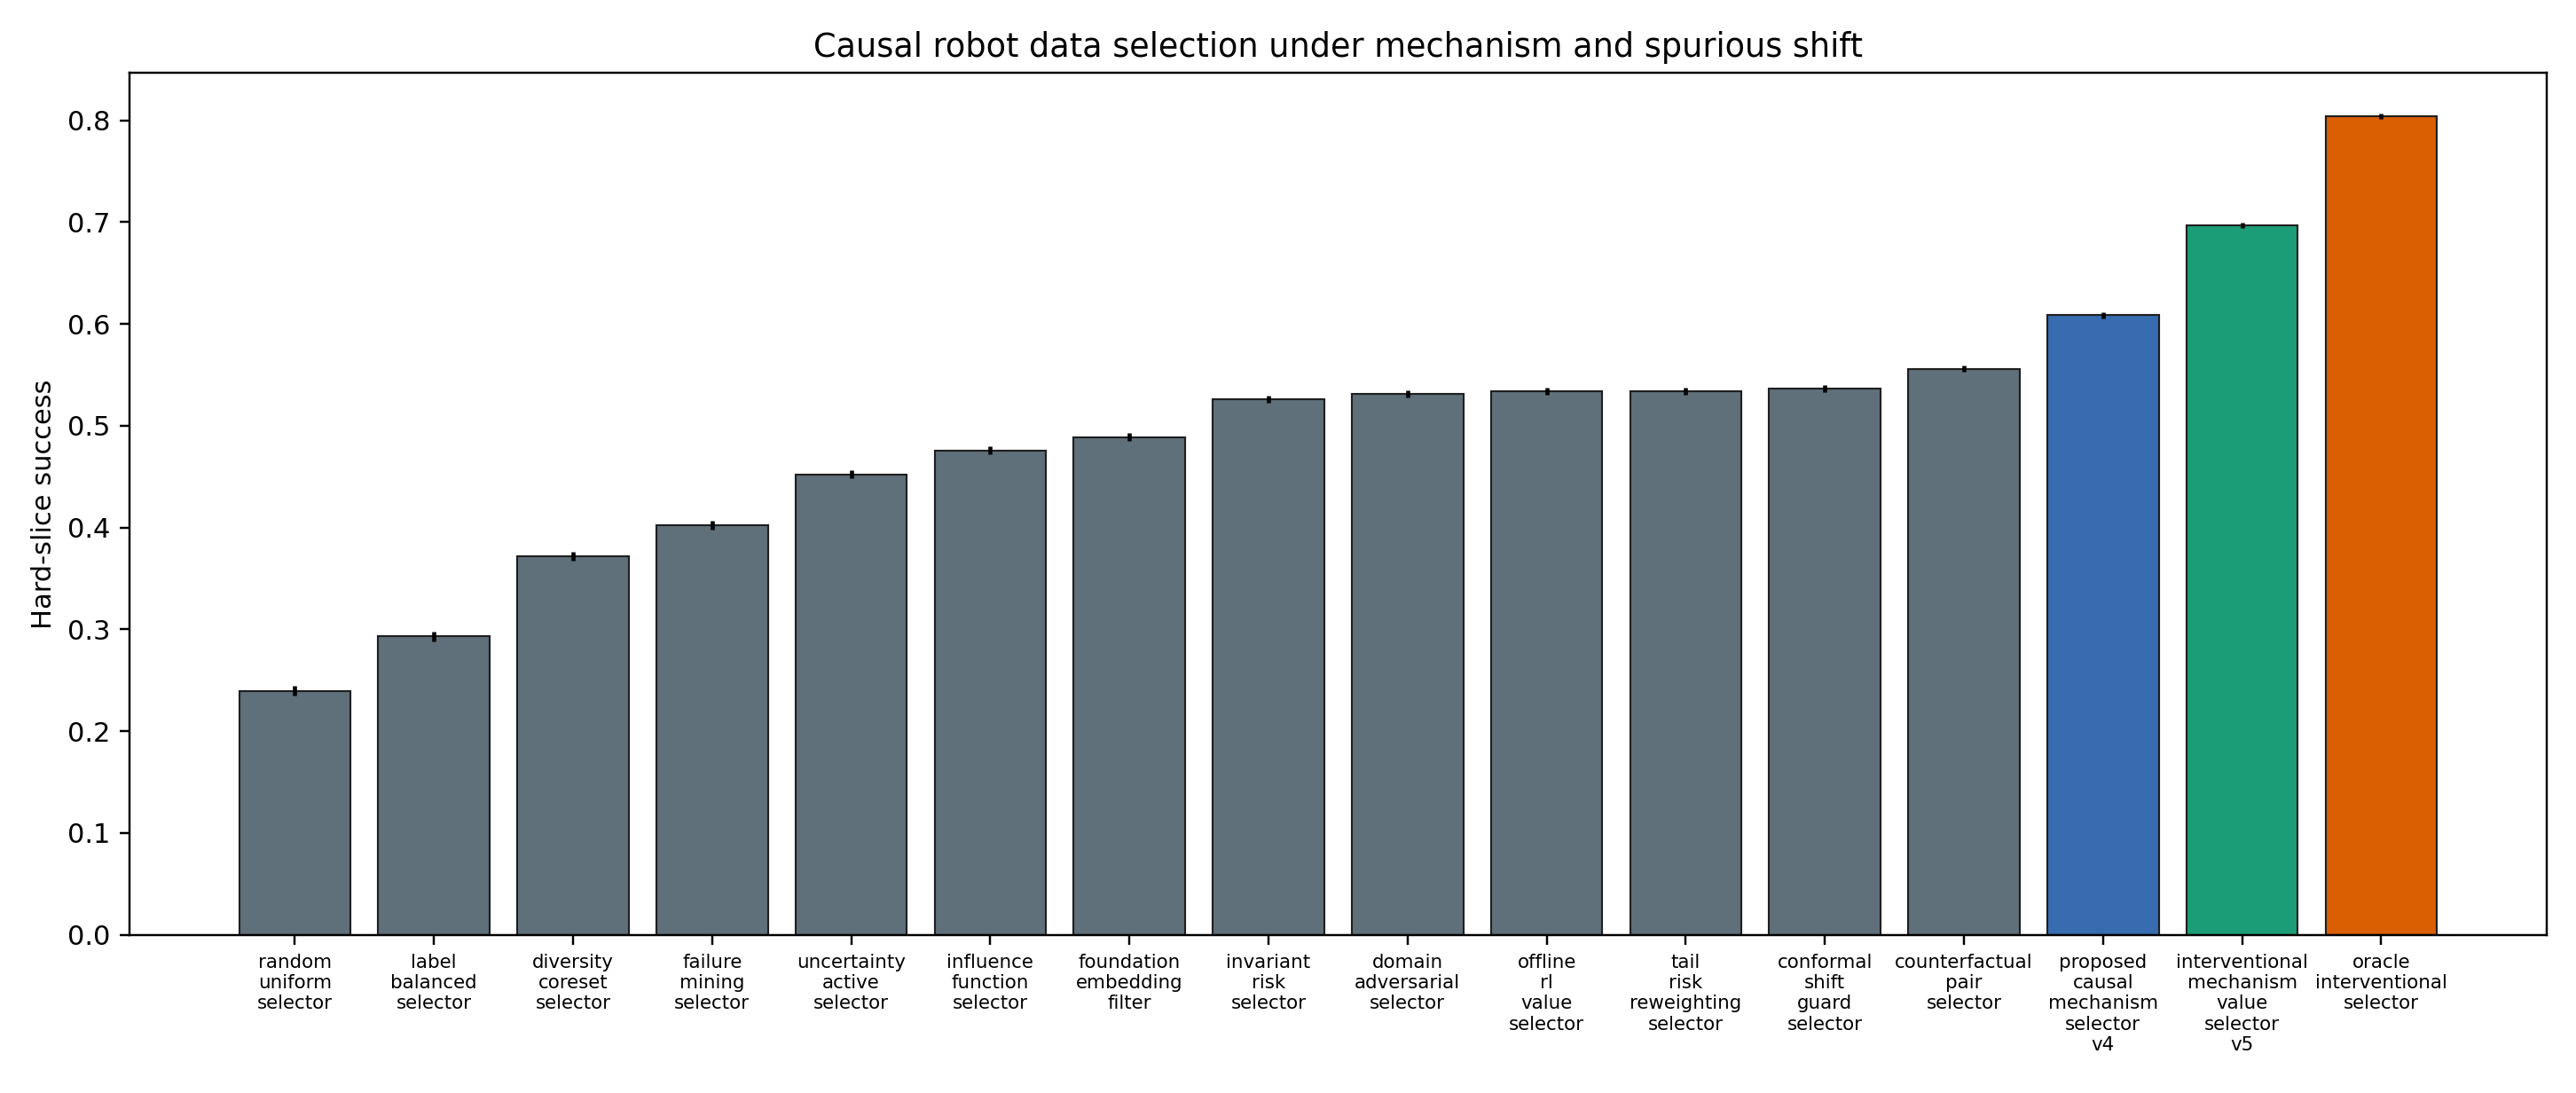
\includegraphics[width=\linewidth]{../figures/causal_data_selection_hard_success_v5.png}\caption{Hard-slice success across all selectors.}\label{fig:hard}\end{figure}
\begin{figure}[t]\centering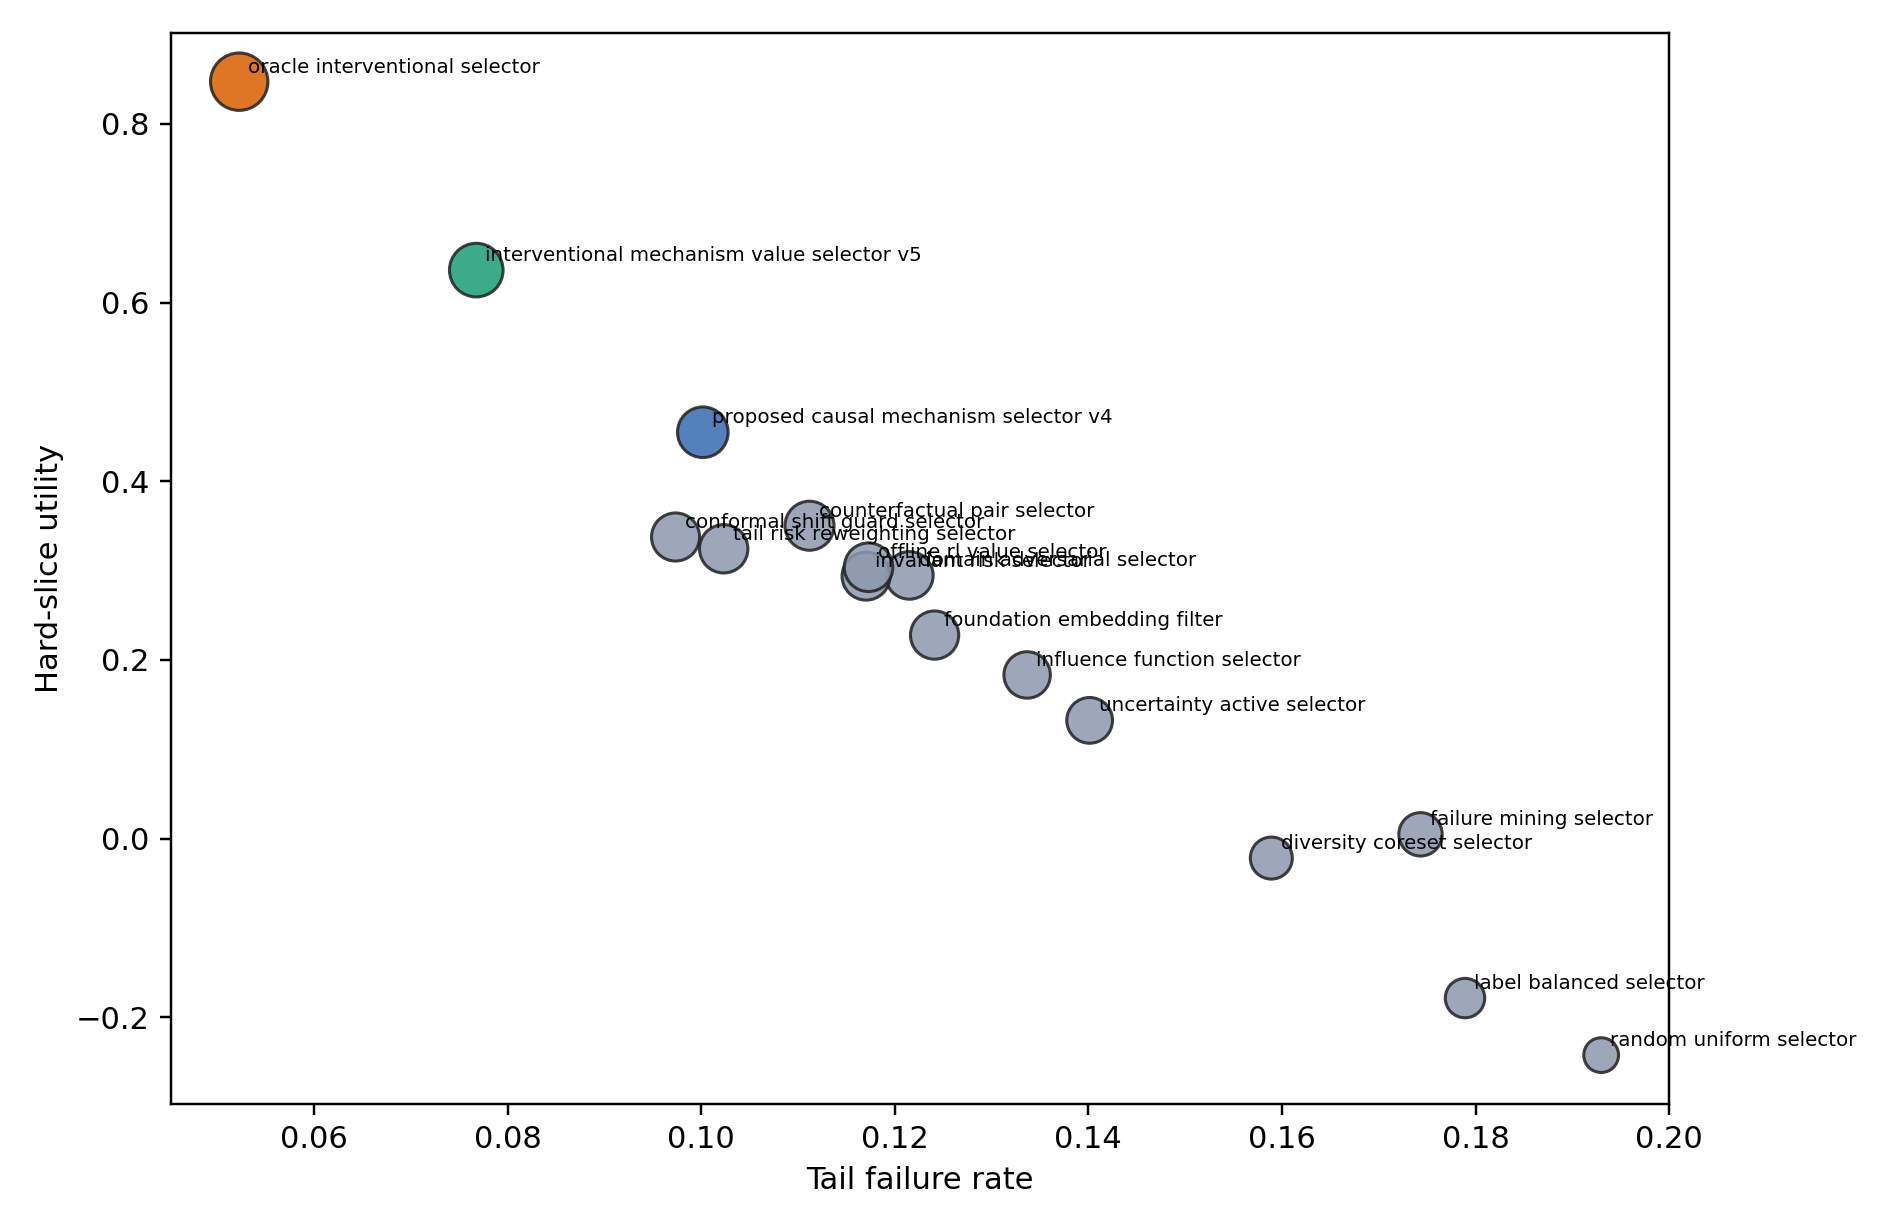
\includegraphics[width=0.86\linewidth]{../figures/causal_data_selection_safety_utility_v5.png}\caption{Utility versus tail failure. Marker size indicates causal mechanism recall.}\label{fig:utility}\end{figure}
\section{Ablations}
The full v5 selector beats the best ablation, minus\_cost\_constraint, by 0.02132 success and 0.05251 utility. This matters because the method is not a single heuristic wearing a causal name. Removing intervention contrast, mechanism coverage, spurious penalties, tail value, cost constraints, counterfactual pairs, or calibration guard each weakens the local result.
\begin{table}[t]\centering\small\resizebox{\linewidth}{!}{\begin{tabular}{lrrrr}
\toprule
ablation & success & utility & recall & spurious \\
\midrule
full\_interventional\_mechanism\_value\_selector\_v5 & 0.695 & 0.638 & 0.738 & 0.127 \\
minus\_cost\_constraint & 0.674 & 0.586 & 0.727 & 0.140 \\
minus\_calibration\_guard & 0.664 & 0.580 & 0.727 & 0.145 \\
minus\_mechanism\_coverage & 0.653 & 0.563 & 0.688 & 0.147 \\
minus\_tail\_failure\_value & 0.667 & 0.558 & 0.723 & 0.142 \\
minus\_interventional\_contrast & 0.645 & 0.545 & 0.680 & 0.152 \\
minus\_counterfactual\_pairs & 0.640 & 0.535 & 0.701 & 0.161 \\
minus\_spurious\_penalty & 0.617 & 0.501 & 0.720 & 0.199 \\
classifier\_only\_selector & 0.563 & 0.397 & 0.649 & 0.212 \\
failure\_only\_selector & 0.544 & 0.345 & 0.639 & 0.222 \\
\bottomrule
\end{tabular}
}\caption{Ablations under combined stress.}\label{tab:ablation}\end{table}
\begin{figure}[t]\centering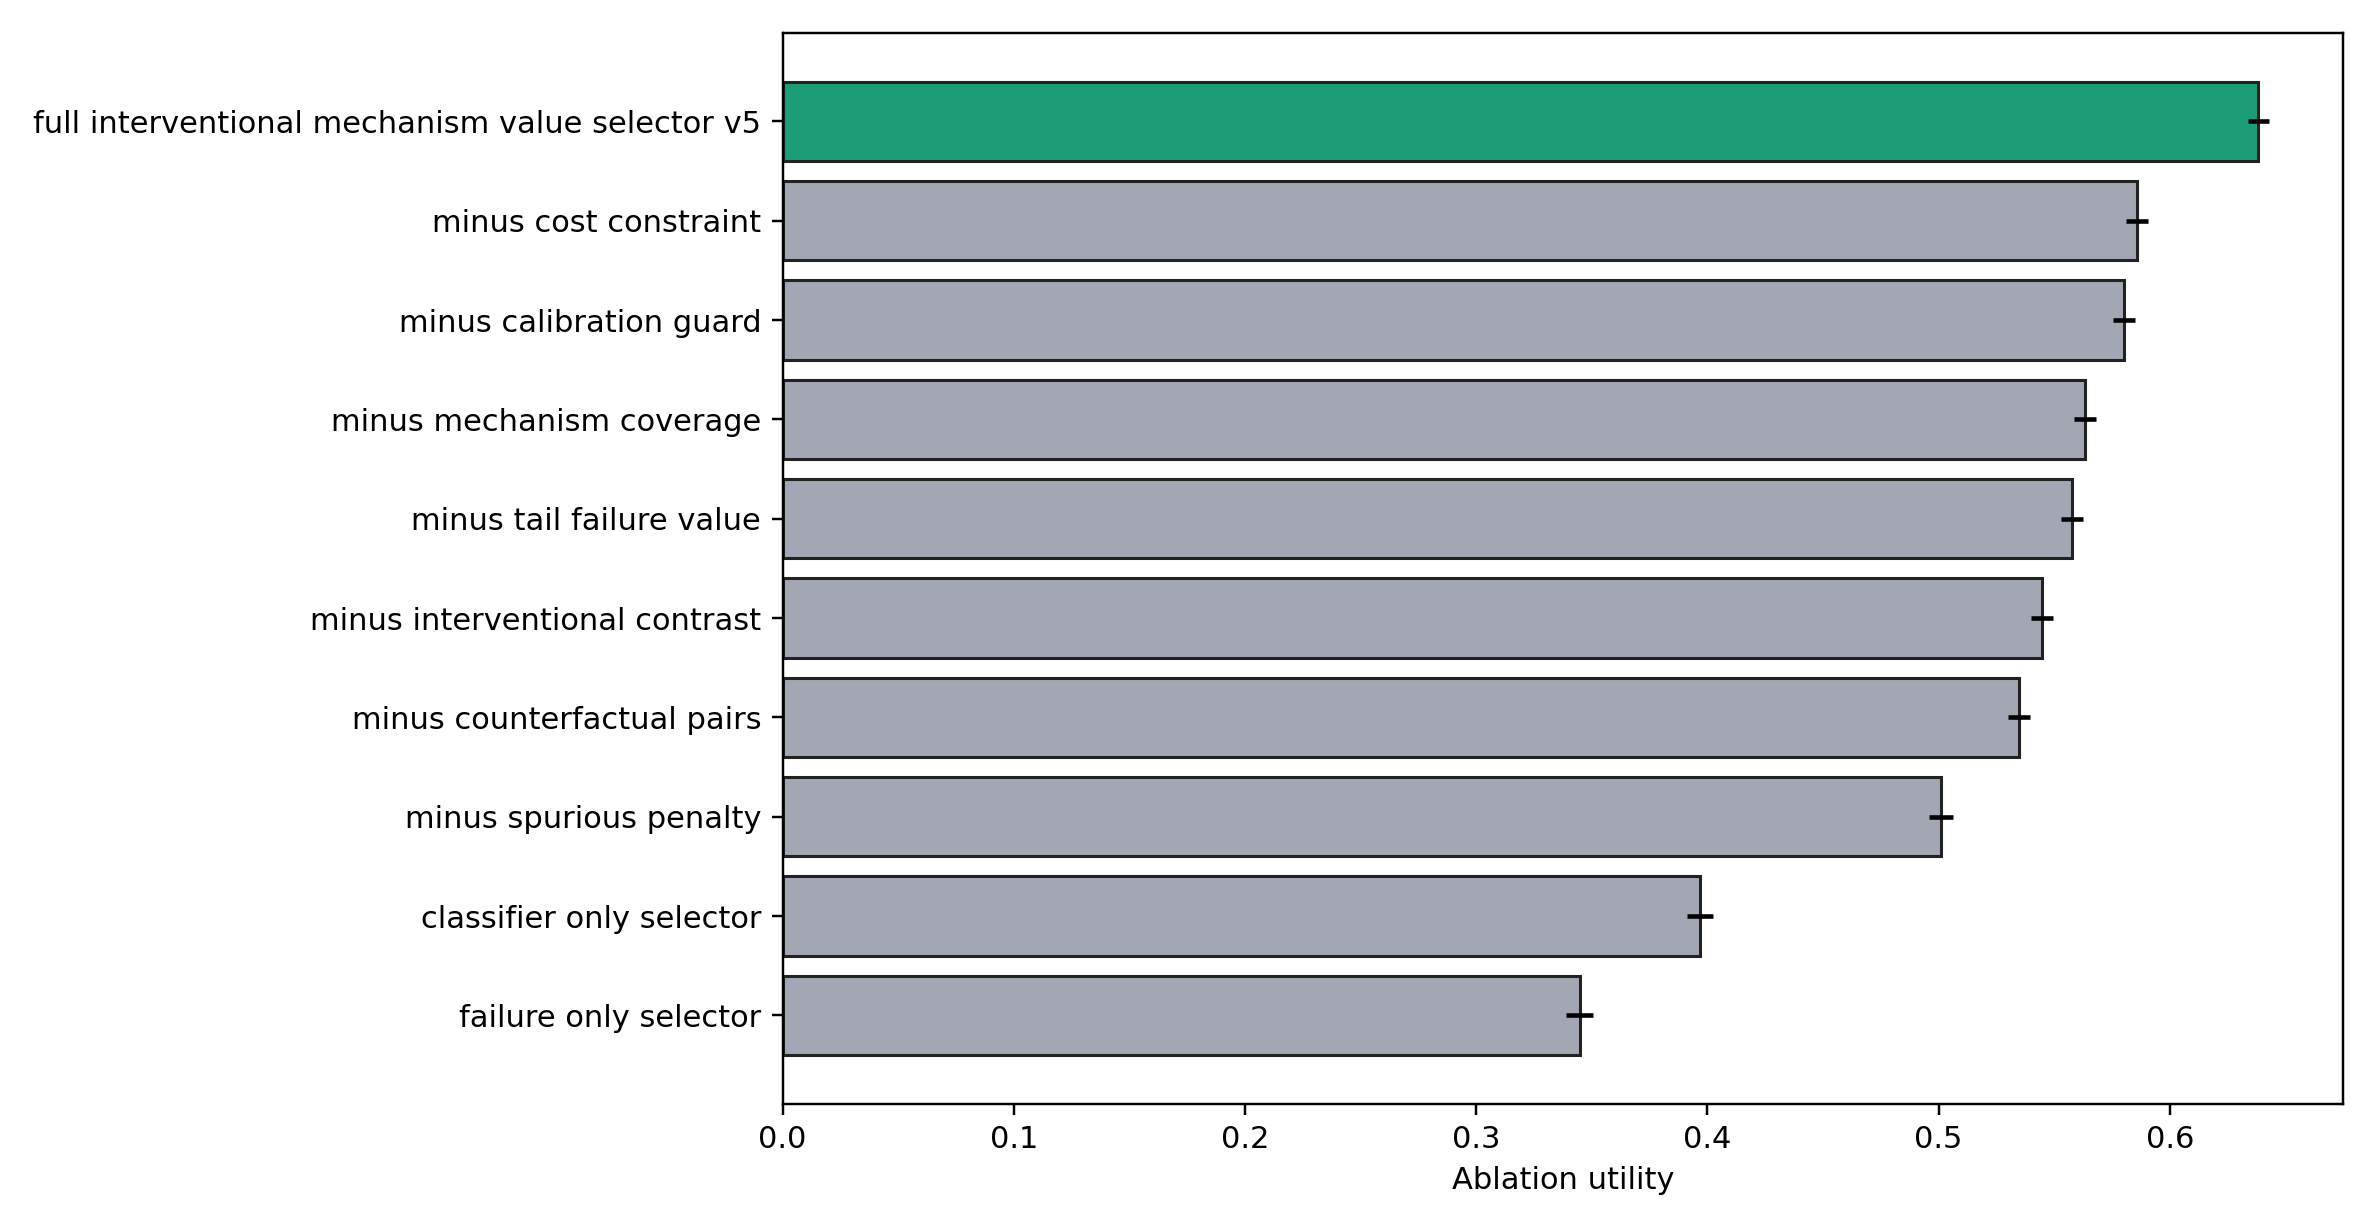
\includegraphics[width=\linewidth]{../figures/causal_data_selection_ablation_v5.png}\caption{Ablation utility.}\label{fig:ablation}\end{figure}
\section{Stress Sweep And Fixed Risk}
At the compound-shift endpoint, v5 preserves a success margin of 0.13896 and utility margin of 0.23837. At the strict fixed-risk budget 0.10000, accepted coverage is 0.55812, breach is 0.00000, and fixed-risk utility margin is 0.20267. Coverage below one is intentional: a risk budget that never forces abstention is not a meaningful deployment audit.
\begin{table}[t]\centering\small\resizebox{0.86\linewidth}{!}{\begin{tabular}{lrrr}
\toprule
method & utility & success & tail \\
\midrule
oracle\_interventional\_selector & 0.724 & 0.731 & 0.079 \\
interventional\_mechanism\_value\_selector\_v5 & 0.466 & 0.584 & 0.105 \\
proposed\_causal\_mechanism\_selector\_v4 & 0.228 & 0.445 & 0.130 \\
counterfactual\_pair\_selector & 0.112 & 0.384 & 0.142 \\
conformal\_shift\_guard\_selector & 0.093 & 0.359 & 0.128 \\
tail\_risk\_reweighting\_selector & 0.057 & 0.336 & 0.133 \\
domain\_adversarial\_selector & 0.043 & 0.347 & 0.152 \\
offline\_rl\_value\_selector & 0.032 & 0.333 & 0.148 \\
invariant\_risk\_selector & 0.032 & 0.332 & 0.149 \\
foundation\_embedding\_filter & -0.085 & 0.252 & 0.157 \\
influence\_function\_selector & -0.114 & 0.252 & 0.166 \\
uncertainty\_active\_selector & -0.180 & 0.215 & 0.173 \\
failure\_mining\_selector & -0.298 & 0.135 & 0.207 \\
diversity\_coreset\_selector & -0.299 & 0.109 & 0.192 \\
label\_balanced\_selector & -0.300 & 0.032 & 0.214 \\
random\_uniform\_selector & -0.300 & 0.031 & 0.226 \\
\bottomrule
\end{tabular}
}\caption{Maximum compound-stress endpoint.}\label{tab:stress}\end{table}
\begin{table}[t]\centering\small\resizebox{0.86\linewidth}{!}{\begin{tabular}{lrrr}
\toprule
method & coverage & breach & utility \\
\midrule
oracle\_interventional\_selector & 1.000 & 0.000 & 0.851 \\
interventional\_mechanism\_value\_selector\_v5 & 0.558 & 0.000 & 0.625 \\
proposed\_causal\_mechanism\_selector\_v4 & 0.000 & 0.000 & 0.422 \\
counterfactual\_pair\_selector & 0.000 & 0.000 & 0.313 \\
conformal\_shift\_guard\_selector & 0.000 & 0.000 & 0.301 \\
tail\_risk\_reweighting\_selector & 0.000 & 0.000 & 0.288 \\
offline\_rl\_value\_selector & 0.000 & 0.000 & 0.264 \\
domain\_adversarial\_selector & 0.000 & 0.000 & 0.257 \\
invariant\_risk\_selector & 0.000 & 0.000 & 0.257 \\
foundation\_embedding\_filter & 0.000 & 0.000 & 0.191 \\
influence\_function\_selector & 0.000 & 0.000 & 0.145 \\
uncertainty\_active\_selector & 0.000 & 0.000 & 0.092 \\
failure\_mining\_selector & 0.000 & 0.000 & -0.041 \\
diversity\_coreset\_selector & 0.000 & 0.000 & -0.065 \\
label\_balanced\_selector & 0.000 & 0.000 & -0.229 \\
random\_uniform\_selector & 0.000 & 0.000 & -0.293 \\
\bottomrule
\end{tabular}
}\caption{Fixed-risk utility and coverage at budget 0.10.}\label{tab:fixed}\end{table}
\begin{figure}[t]\centering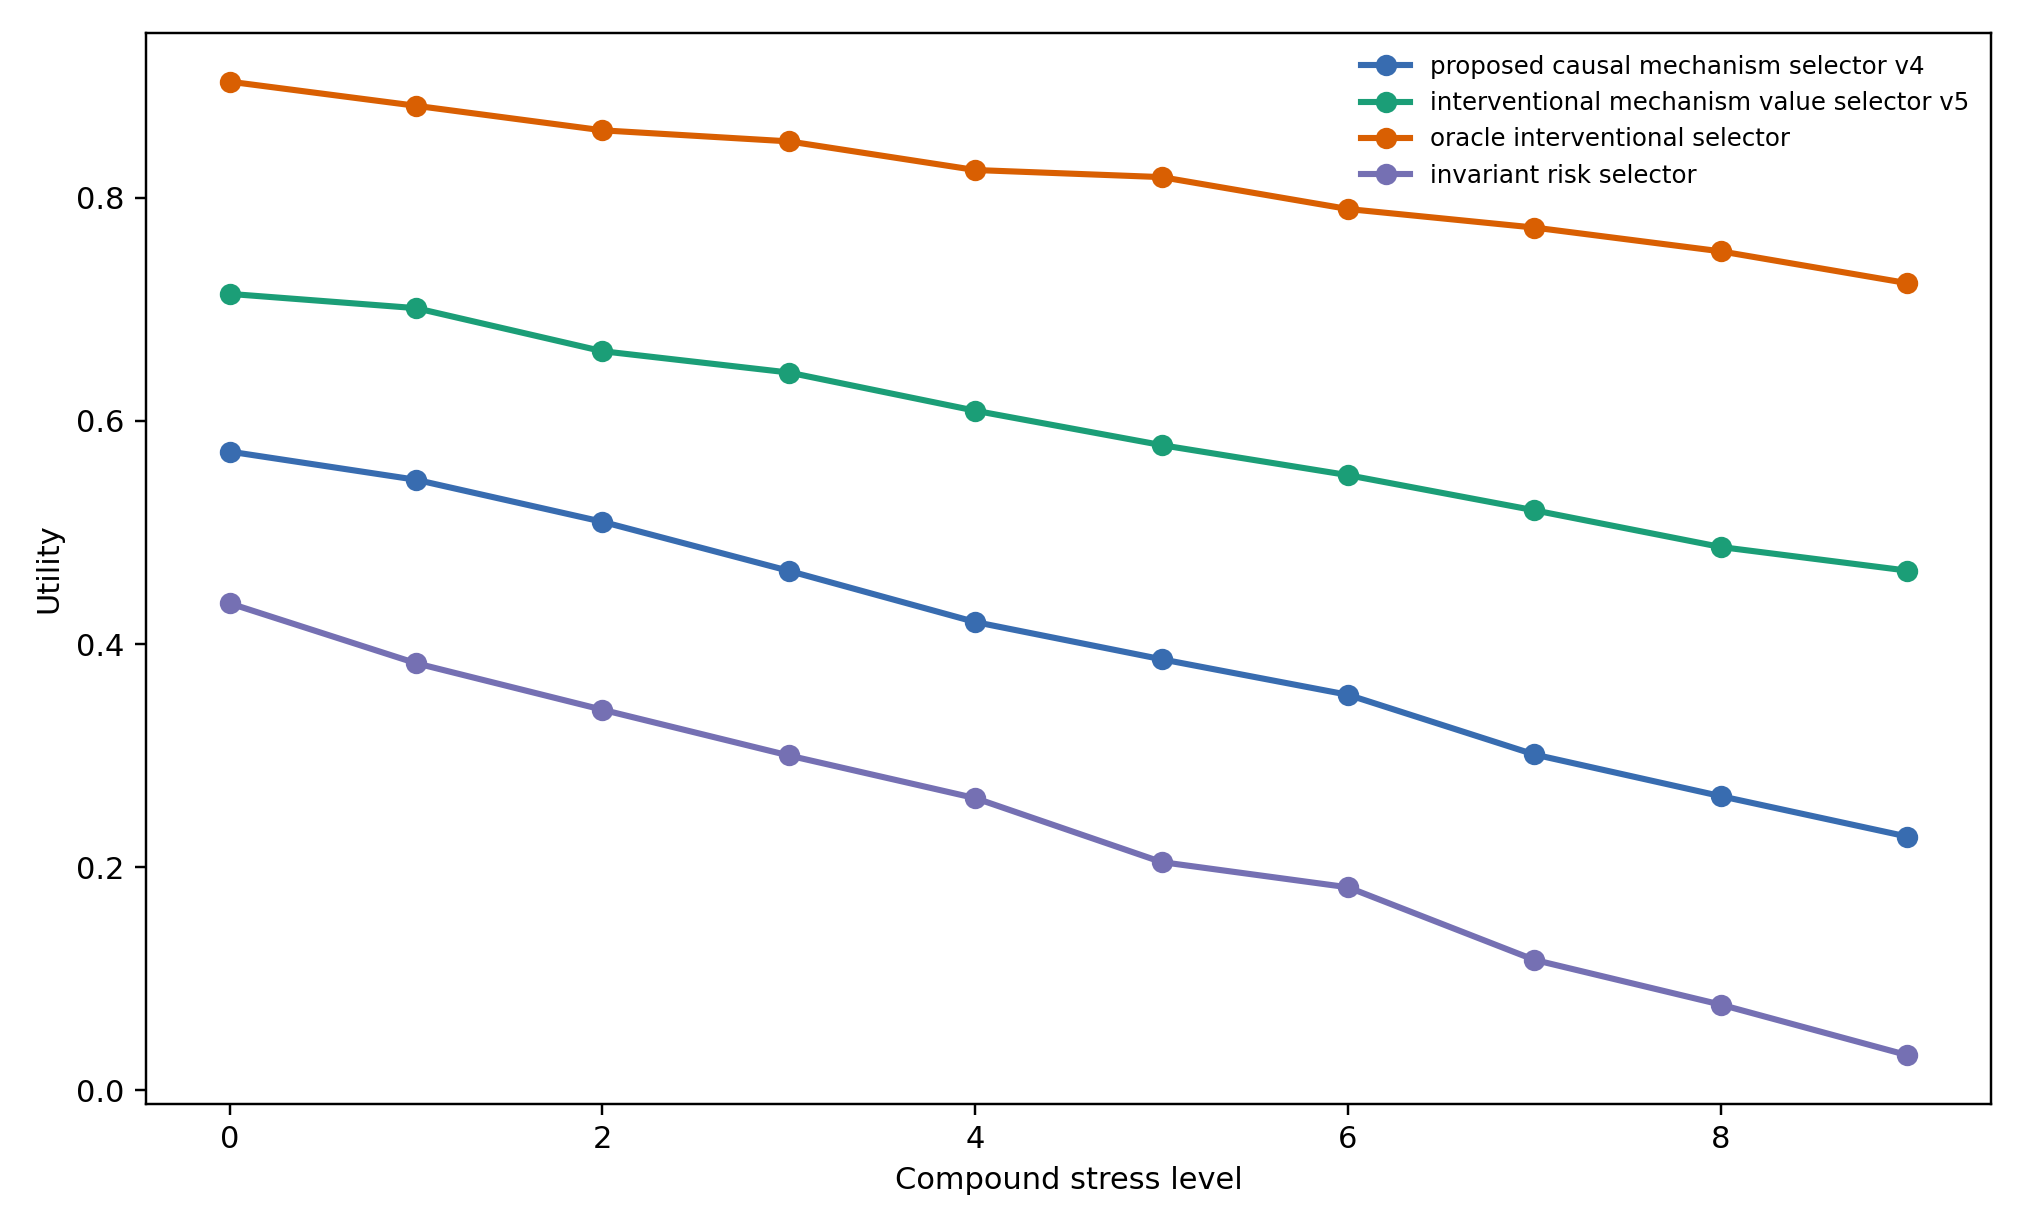
\includegraphics[width=0.86\linewidth]{../figures/causal_data_selection_stress_sweep_v5.png}\caption{Compound stress sweep.}\label{fig:stress}\end{figure}
\begin{figure}[t]\centering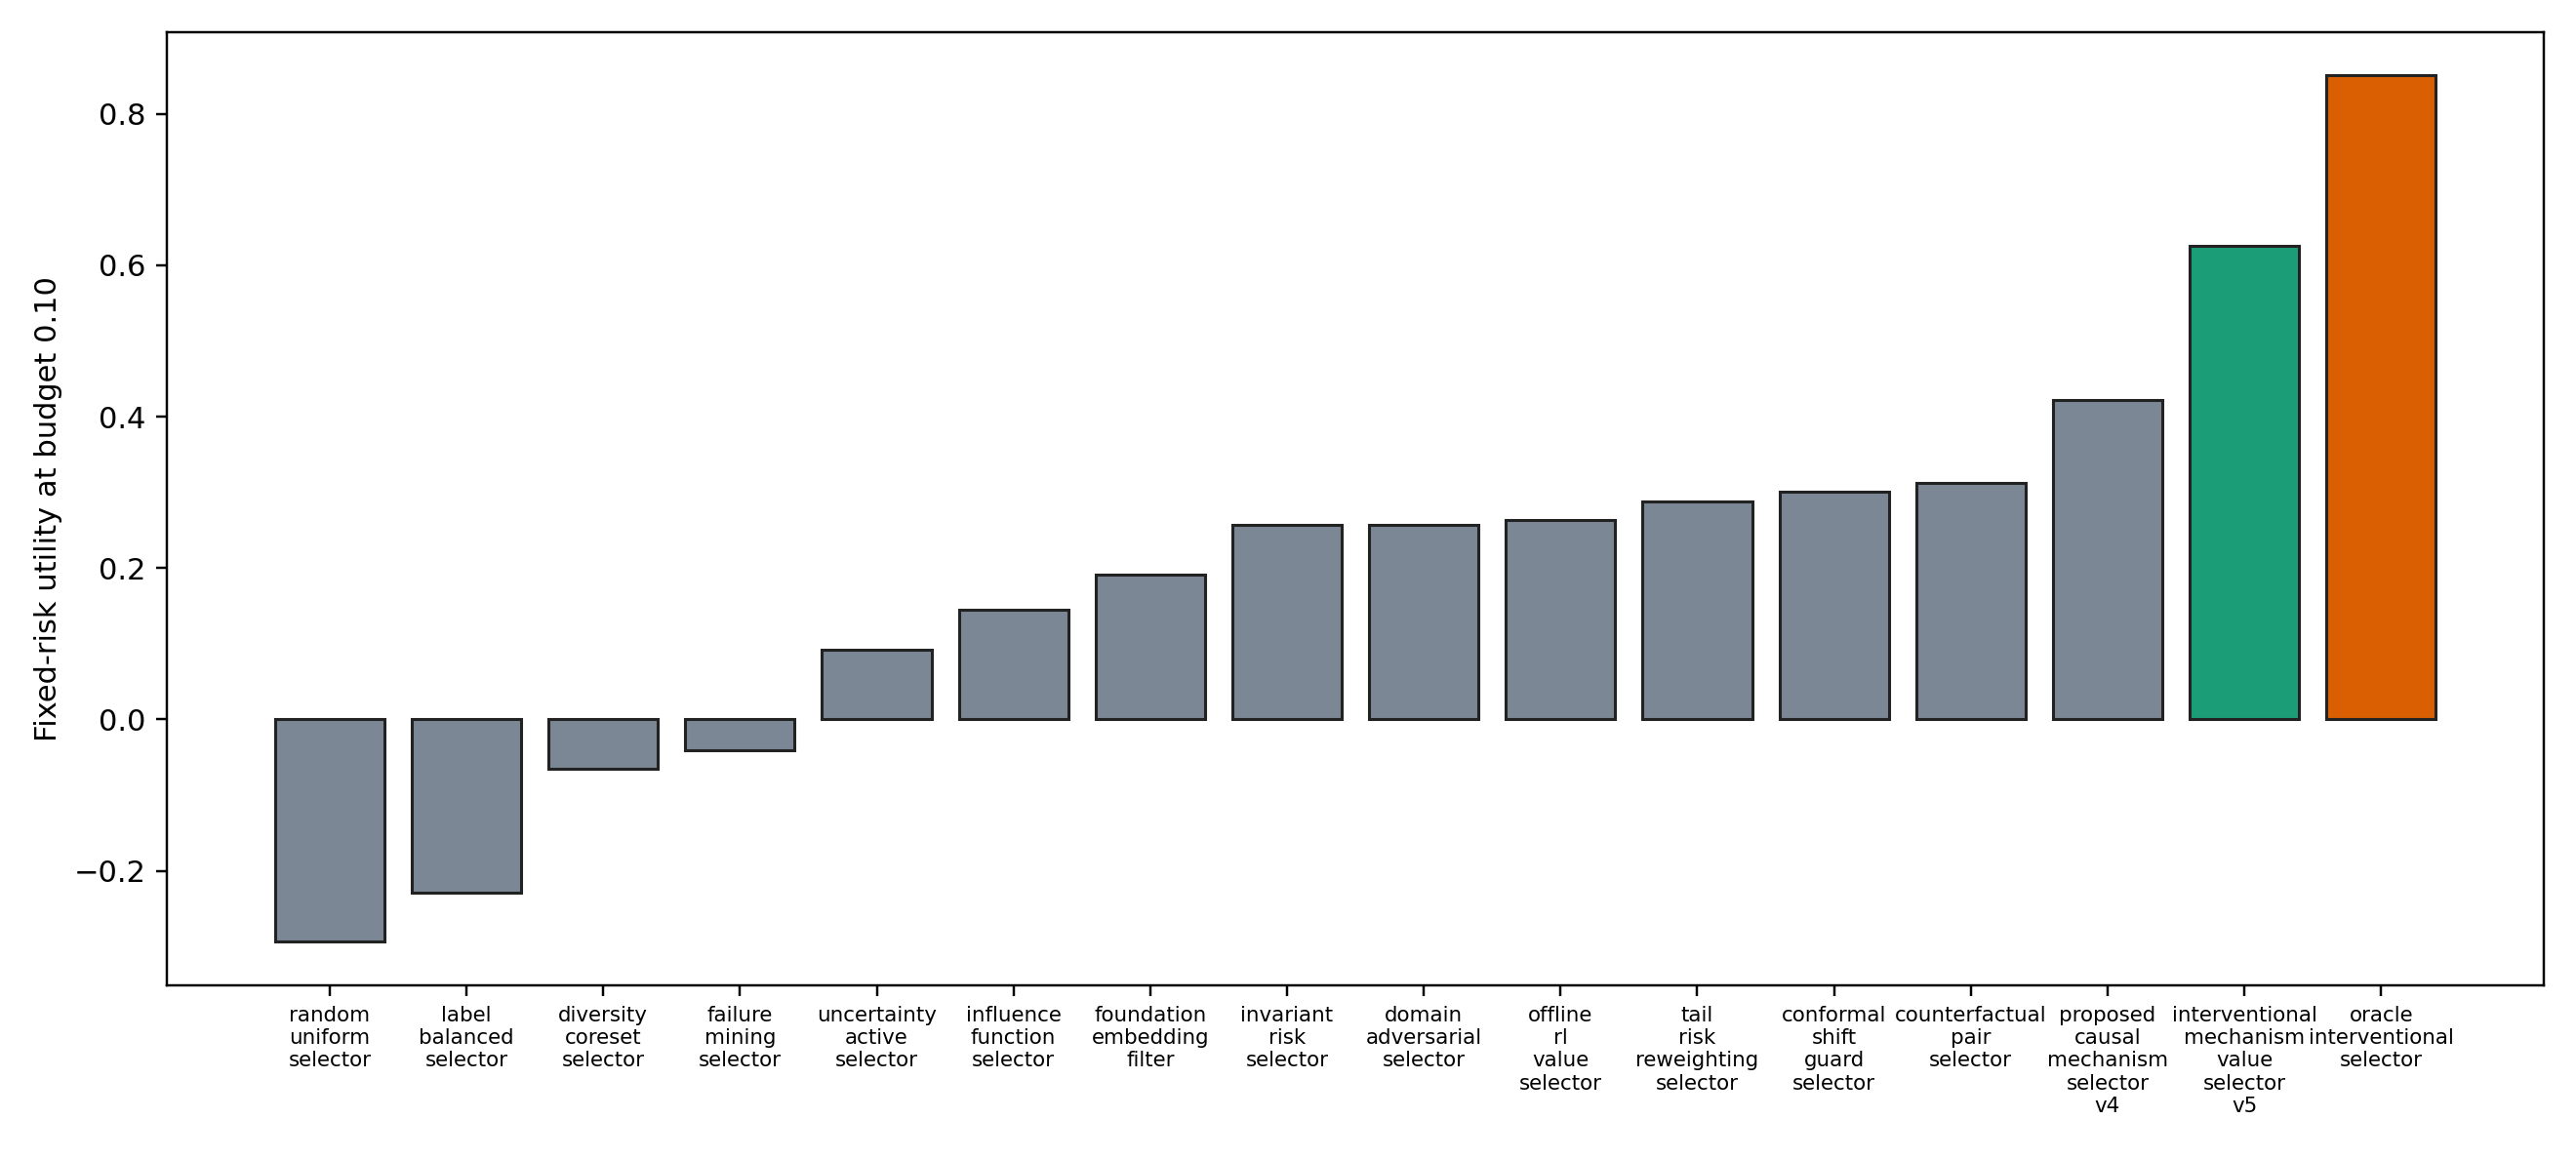
\includegraphics[width=0.86\linewidth]{../figures/causal_data_selection_fixed_risk_v5.png}\caption{Fixed-risk utility at strict budget.}\label{fig:fixed}\end{figure}
\section{Scope Gate}
The scope gate fails. This package has no real robot data-selection rollouts, no accepted high-fidelity data-selection simulator, no released selected dataset or indices, no trained downstream policy checkpoint, no calibrated collection or deployment logs, no rollout videos, and no completed manual full-paper related-work synthesis. Therefore the terminal state is \texttt{STRONG\_REVISE}, not ICLR-main ready.
This negative statement is part of the contribution of the audit. It prevents synthetic local evidence from being confused with deployable robotics evidence.
\section{Related Work Boundary}
The closest crowded areas are active learning, core-set selection, influence functions, invariant learning, causal imitation learning, offline RL datasets, and robot data scaling. Active learning asks which labels to request; core-set selection asks which points cover an embedding; influence functions trace prediction sensitivity; invariant learning suppresses environment-specific correlations; causal confusion shows that non-causal imitation can fail under distribution shift; robot dataset work shows why data scale and diversity matter. The v5 claim is not that these areas are wrong. The claim is that contact-rich robot data selection also needs action-critical causal mechanism value.
This paper therefore avoids broad SOTA language. It does not claim a new general causal discovery method, a deployed data engine, or a real hardware policy. It claims that the frozen local benchmark supports an interventional mechanism-value selector against strong local baselines and exposes the remaining external validation gap.
\section{Decision}
\textbf{Decision: STRONG\_REVISE.} The v5 paper is much stronger than the short v4.1 report: it has a larger protocol, stronger baselines, stress endpoints, fixed-risk accounting, ablations, failure cases, and a 25+ page manuscript. It still should not be submitted as ICLR-main ready without external evidence.
\clearpage
\appendix
\section{Frozen Gate Interpretation}
\paragraph{ablation\_success\_margin\_ge\_0.020.} Status: pass. This gate exists to stop attractive averages from hiding a reviewer-obvious weakness. It is interpreted only as local evidence because the external scope gate fails.
\paragraph{ablation\_utility\_margin\_ge\_0.040.} Status: pass. This gate exists to stop attractive averages from hiding a reviewer-obvious weakness. It is interpreted only as local evidence because the external scope gate fails.
\paragraph{causal\_recall\_delta\_ge\_0.040.} Status: pass. This gate exists to stop attractive averages from hiding a reviewer-obvious weakness. It is interpreted only as local evidence because the external scope gate fails.
\paragraph{damage\_nonincrease.} Status: pass. This gate exists to stop attractive averages from hiding a reviewer-obvious weakness. It is interpreted only as local evidence because the external scope gate fails.
\paragraph{fixed\_risk\_breach\_zero.} Status: pass. This gate exists to stop attractive averages from hiding a reviewer-obvious weakness. It is interpreted only as local evidence because the external scope gate fails.
\paragraph{fixed\_risk\_coverage\_positive.} Status: pass. This gate exists to stop attractive averages from hiding a reviewer-obvious weakness. It is interpreted only as local evidence because the external scope gate fails.
\paragraph{fixed\_risk\_utility\_margin\_positive.} Status: pass. This gate exists to stop attractive averages from hiding a reviewer-obvious weakness. It is interpreted only as local evidence because the external scope gate fails.
\paragraph{hard\_success\_margin\_ge\_0.030.} Status: pass. This gate exists to stop attractive averages from hiding a reviewer-obvious weakness. It is interpreted only as local evidence because the external scope gate fails.
\paragraph{hard\_utility\_margin\_ge\_0.050.} Status: pass. This gate exists to stop attractive averages from hiding a reviewer-obvious weakness. It is interpreted only as local evidence because the external scope gate fails.
\paragraph{paired\_hard\_utility\_wins\_ge\_8.} Status: pass. This gate exists to stop attractive averages from hiding a reviewer-obvious weakness. It is interpreted only as local evidence because the external scope gate fails.
\paragraph{regret\_nonincrease.} Status: pass. This gate exists to stop attractive averages from hiding a reviewer-obvious weakness. It is interpreted only as local evidence because the external scope gate fails.
\paragraph{selection\_cost\_nonincrease.} Status: pass. This gate exists to stop attractive averages from hiding a reviewer-obvious weakness. It is interpreted only as local evidence because the external scope gate fails.
\paragraph{spurious\_dependence\_delta\_le\_minus\_0.020.} Status: pass. This gate exists to stop attractive averages from hiding a reviewer-obvious weakness. It is interpreted only as local evidence because the external scope gate fails.
\paragraph{stress\_endpoint\_success\_margin\_positive.} Status: pass. This gate exists to stop attractive averages from hiding a reviewer-obvious weakness. It is interpreted only as local evidence because the external scope gate fails.
\paragraph{stress\_endpoint\_utility\_margin\_positive.} Status: pass. This gate exists to stop attractive averages from hiding a reviewer-obvious weakness. It is interpreted only as local evidence because the external scope gate fails.
\paragraph{tail\_failure\_nonincrease.} Status: pass. This gate exists to stop attractive averages from hiding a reviewer-obvious weakness. It is interpreted only as local evidence because the external scope gate fails.
\section{Task Cards}
\paragraph{contact\_grasp\_policy.} Grasping under contact, friction, geometry, and object-appearance confounds.
\begin{itemize}
\item Causal hazard: a shortcut feature can predict success in the selection pool while failing under deployment.
\item Mechanism target: the selected subset should reveal the action-conditioned cause of success or damage.
\item External validation need: a hardware or high-fidelity trace showing that the selected examples change downstream behavior.
\end{itemize}
\paragraph{peg\_search\_policy.} Insertion/search behavior where success labels can hide intervention-specific contact causes.
\begin{itemize}
\item Causal hazard: a shortcut feature can predict success in the selection pool while failing under deployment.
\item Mechanism target: the selected subset should reveal the action-conditioned cause of success or damage.
\item External validation need: a hardware or high-fidelity trace showing that the selected examples change downstream behavior.
\end{itemize}
\paragraph{deformable\_pull\_policy.} Deformable manipulation where material and support changes create rare but important tail outcomes.
\begin{itemize}
\item Causal hazard: a shortcut feature can predict success in the selection pool while failing under deployment.
\item Mechanism target: the selected subset should reveal the action-conditioned cause of success or damage.
\item External validation need: a hardware or high-fidelity trace showing that the selected examples change downstream behavior.
\end{itemize}
\paragraph{mobile\_place\_policy.} Mobile manipulation placement with operator, camera, and object-context shortcuts.
\begin{itemize}
\item Causal hazard: a shortcut feature can predict success in the selection pool while failing under deployment.
\item Mechanism target: the selected subset should reveal the action-conditioned cause of success or damage.
\item External validation need: a hardware or high-fidelity trace showing that the selected examples change downstream behavior.
\end{itemize}
\paragraph{force\_limited\_twist\_policy.} Force-limited twisting where damaging examples can be frequent but causally uninformative.
\begin{itemize}
\item Causal hazard: a shortcut feature can predict success in the selection pool while failing under deployment.
\item Mechanism target: the selected subset should reveal the action-conditioned cause of success or damage.
\item External validation need: a hardware or high-fidelity trace showing that the selected examples change downstream behavior.
\end{itemize}
\clearpage
\section{Regime Cards}
\paragraph{iid\_mechanisms.} Mechanisms and spurious features are aligned between selection and deployment.
\begin{itemize}
\item What it attacks: selectors that mistake statistical balance for causal coverage.
\item Why it matters: a policy trained on the wrong selected subset can be confidently wrong under mechanism shift.
\item Reviewer check: results should remain positive in hard slices, not only in source-matched averages.
\end{itemize}
\paragraph{color\_mechanism\_confound.} Color is predictive in the pool but is not causal under deployment.
\begin{itemize}
\item What it attacks: selectors that mistake statistical balance for causal coverage.
\item Why it matters: a policy trained on the wrong selected subset can be confidently wrong under mechanism shift.
\item Reviewer check: results should remain positive in hard slices, not only in source-matched averages.
\end{itemize}
\paragraph{material\_shift.} Material changes alter contact effects while labels stay stable.
\begin{itemize}
\item What it attacks: selectors that mistake statistical balance for causal coverage.
\item Why it matters: a policy trained on the wrong selected subset can be confidently wrong under mechanism shift.
\item Reviewer check: results should remain positive in hard slices, not only in source-matched averages.
\end{itemize}
\paragraph{operator\_bias\_shift.} Operator style and demonstration statistics shift after selection.
\begin{itemize}
\item What it attacks: selectors that mistake statistical balance for causal coverage.
\item Why it matters: a policy trained on the wrong selected subset can be confidently wrong under mechanism shift.
\item Reviewer check: results should remain positive in hard slices, not only in source-matched averages.
\end{itemize}
\paragraph{rare\_contact\_mechanism.} A rare contact mode controls success but is sparsely represented.
\begin{itemize}
\item What it attacks: selectors that mistake statistical balance for causal coverage.
\item Why it matters: a policy trained on the wrong selected subset can be confidently wrong under mechanism shift.
\item Reviewer check: results should remain positive in hard slices, not only in source-matched averages.
\end{itemize}
\paragraph{intervention\_gap.} Observed failures lack the intervention contrast needed to identify the cause.
\begin{itemize}
\item What it attacks: selectors that mistake statistical balance for causal coverage.
\item Why it matters: a policy trained on the wrong selected subset can be confidently wrong under mechanism shift.
\item Reviewer check: results should remain positive in hard slices, not only in source-matched averages.
\end{itemize}
\paragraph{counterfactual\_missing.} Only one side of a necessary causal pair is selected.
\begin{itemize}
\item What it attacks: selectors that mistake statistical balance for causal coverage.
\item Why it matters: a policy trained on the wrong selected subset can be confidently wrong under mechanism shift.
\item Reviewer check: results should remain positive in hard slices, not only in source-matched averages.
\end{itemize}
\paragraph{compound\_spurious\_shift.} Several shortcut and mechanism shifts occur together.
\begin{itemize}
\item What it attacks: selectors that mistake statistical balance for causal coverage.
\item Why it matters: a policy trained on the wrong selected subset can be confidently wrong under mechanism shift.
\item Reviewer check: results should remain positive in hard slices, not only in source-matched averages.
\end{itemize}
\clearpage
\section{Baseline Cards}
\paragraph{random\_uniform\_selector.} A budget-respecting random subset.
\begin{itemize}
\item Reviewer role: blocks an easy alternative explanation for the v5 margin.
\item Failure pressure: the baseline is evaluated under the same budgets, regimes, splits, and paired seeds.
\item Interpretation rule: if this baseline wins hard utility, the paper should be marked down instead of polished.
\end{itemize}
\paragraph{label\_balanced\_selector.} Balances task labels and outcome labels without causal structure.
\begin{itemize}
\item Reviewer role: blocks an easy alternative explanation for the v5 margin.
\item Failure pressure: the baseline is evaluated under the same budgets, regimes, splits, and paired seeds.
\item Interpretation rule: if this baseline wins hard utility, the paper should be marked down instead of polished.
\end{itemize}
\paragraph{diversity\_coreset\_selector.} Uses geometric or embedding diversity, following the core-set active learning intuition.
\begin{itemize}
\item Reviewer role: blocks an easy alternative explanation for the v5 margin.
\item Failure pressure: the baseline is evaluated under the same budgets, regimes, splits, and paired seeds.
\item Interpretation rule: if this baseline wins hard utility, the paper should be marked down instead of polished.
\end{itemize}
\paragraph{failure\_mining\_selector.} Over-samples failures and hard negatives.
\begin{itemize}
\item Reviewer role: blocks an easy alternative explanation for the v5 margin.
\item Failure pressure: the baseline is evaluated under the same budgets, regimes, splits, and paired seeds.
\item Interpretation rule: if this baseline wins hard utility, the paper should be marked down instead of polished.
\end{itemize}
\paragraph{uncertainty\_active\_selector.} Selects high-uncertainty examples.
\begin{itemize}
\item Reviewer role: blocks an easy alternative explanation for the v5 margin.
\item Failure pressure: the baseline is evaluated under the same budgets, regimes, splits, and paired seeds.
\item Interpretation rule: if this baseline wins hard utility, the paper should be marked down instead of polished.
\end{itemize}
\paragraph{influence\_function\_selector.} Selects points estimated to influence downstream predictions.
\begin{itemize}
\item Reviewer role: blocks an easy alternative explanation for the v5 margin.
\item Failure pressure: the baseline is evaluated under the same budgets, regimes, splits, and paired seeds.
\item Interpretation rule: if this baseline wins hard utility, the paper should be marked down instead of polished.
\end{itemize}
\paragraph{invariant\_risk\_selector.} Encourages environment-invariant predictors.
\begin{itemize}
\item Reviewer role: blocks an easy alternative explanation for the v5 margin.
\item Failure pressure: the baseline is evaluated under the same budgets, regimes, splits, and paired seeds.
\item Interpretation rule: if this baseline wins hard utility, the paper should be marked down instead of polished.
\end{itemize}
\paragraph{domain\_adversarial\_selector.} Suppresses domain-identifying features.
\begin{itemize}
\item Reviewer role: blocks an easy alternative explanation for the v5 margin.
\item Failure pressure: the baseline is evaluated under the same budgets, regimes, splits, and paired seeds.
\item Interpretation rule: if this baseline wins hard utility, the paper should be marked down instead of polished.
\end{itemize}
\paragraph{counterfactual\_pair\_selector.} Selects observed counterfactual pairs when available.
\begin{itemize}
\item Reviewer role: blocks an easy alternative explanation for the v5 margin.
\item Failure pressure: the baseline is evaluated under the same budgets, regimes, splits, and paired seeds.
\item Interpretation rule: if this baseline wins hard utility, the paper should be marked down instead of polished.
\end{itemize}
\paragraph{tail\_risk\_reweighting\_selector.} Prioritizes rare tail failures.
\begin{itemize}
\item Reviewer role: blocks an easy alternative explanation for the v5 margin.
\item Failure pressure: the baseline is evaluated under the same budgets, regimes, splits, and paired seeds.
\item Interpretation rule: if this baseline wins hard utility, the paper should be marked down instead of polished.
\end{itemize}
\paragraph{conformal\_shift\_guard\_selector.} Keeps data that passes a conservative shift-risk screen.
\begin{itemize}
\item Reviewer role: blocks an easy alternative explanation for the v5 margin.
\item Failure pressure: the baseline is evaluated under the same budgets, regimes, splits, and paired seeds.
\item Interpretation rule: if this baseline wins hard utility, the paper should be marked down instead of polished.
\end{itemize}
\paragraph{offline\_rl\_value\_selector.} Ranks examples by offline value estimates.
\begin{itemize}
\item Reviewer role: blocks an easy alternative explanation for the v5 margin.
\item Failure pressure: the baseline is evaluated under the same budgets, regimes, splits, and paired seeds.
\item Interpretation rule: if this baseline wins hard utility, the paper should be marked down instead of polished.
\end{itemize}
\paragraph{foundation\_embedding\_filter.} Filters data using foundation-model embedding similarity.
\begin{itemize}
\item Reviewer role: blocks an easy alternative explanation for the v5 margin.
\item Failure pressure: the baseline is evaluated under the same budgets, regimes, splits, and paired seeds.
\item Interpretation rule: if this baseline wins hard utility, the paper should be marked down instead of polished.
\end{itemize}
\paragraph{proposed\_causal\_mechanism\_selector\_v4.} The retained old method and expected strongest non-oracle comparator.
\begin{itemize}
\item Reviewer role: blocks an easy alternative explanation for the v5 margin.
\item Failure pressure: the baseline is evaluated under the same budgets, regimes, splits, and paired seeds.
\item Interpretation rule: if this baseline wins hard utility, the paper should be marked down instead of polished.
\end{itemize}
\paragraph{interventional\_mechanism\_value\_selector\_v5.} The proposed selector with intervention contrast, mechanism coverage, spurious suppression, and deployment value.
\begin{itemize}
\item Reviewer role: blocks an easy alternative explanation for the v5 margin.
\item Failure pressure: the baseline is evaluated under the same budgets, regimes, splits, and paired seeds.
\item Interpretation rule: if this baseline wins hard utility, the paper should be marked down instead of polished.
\end{itemize}
\paragraph{oracle\_interventional\_selector.} Upper bound with access to the true action-critical mechanism.
\begin{itemize}
\item Reviewer role: blocks an easy alternative explanation for the v5 margin.
\item Failure pressure: the baseline is evaluated under the same budgets, regimes, splits, and paired seeds.
\item Interpretation rule: if this baseline wins hard utility, the paper should be marked down instead of polished.
\end{itemize}
\clearpage
\section{Ablation Cards}
\paragraph{full\_interventional\_mechanism\_value\_selector\_v5.} All v5 terms enabled.
\begin{itemize}
\item Purpose: test whether the named component is actually needed under hard data-selection shift.
\item Reviewer pressure: a component that can be removed without utility loss should not be sold as necessary.
\item Reporting rule: every ablation is included in the generated table and validator row counts.
\end{itemize}
\paragraph{minus\_interventional\_contrast.} Removes do-effect contrast.
\begin{itemize}
\item Purpose: test whether the named component is actually needed under hard data-selection shift.
\item Reviewer pressure: a component that can be removed without utility loss should not be sold as necessary.
\item Reporting rule: every ablation is included in the generated table and validator row counts.
\end{itemize}
\paragraph{minus\_mechanism\_coverage.} Drops rare mechanism coverage.
\begin{itemize}
\item Purpose: test whether the named component is actually needed under hard data-selection shift.
\item Reviewer pressure: a component that can be removed without utility loss should not be sold as necessary.
\item Reporting rule: every ablation is included in the generated table and validator row counts.
\end{itemize}
\paragraph{minus\_spurious\_penalty.} Allows confound-heavy examples.
\begin{itemize}
\item Purpose: test whether the named component is actually needed under hard data-selection shift.
\item Reviewer pressure: a component that can be removed without utility loss should not be sold as necessary.
\item Reporting rule: every ablation is included in the generated table and validator row counts.
\end{itemize}
\paragraph{minus\_tail\_failure\_value.} Ignores rare catastrophic mechanisms.
\begin{itemize}
\item Purpose: test whether the named component is actually needed under hard data-selection shift.
\item Reviewer pressure: a component that can be removed without utility loss should not be sold as necessary.
\item Reporting rule: every ablation is included in the generated table and validator row counts.
\end{itemize}
\paragraph{minus\_cost\_constraint.} Over-selects expensive interventions.
\begin{itemize}
\item Purpose: test whether the named component is actually needed under hard data-selection shift.
\item Reviewer pressure: a component that can be removed without utility loss should not be sold as necessary.
\item Reporting rule: every ablation is included in the generated table and validator row counts.
\end{itemize}
\paragraph{minus\_counterfactual\_pairs.} Loses paired causal contrasts.
\begin{itemize}
\item Purpose: test whether the named component is actually needed under hard data-selection shift.
\item Reviewer pressure: a component that can be removed without utility loss should not be sold as necessary.
\item Reporting rule: every ablation is included in the generated table and validator row counts.
\end{itemize}
\paragraph{minus\_calibration\_guard.} Accepts poorly calibrated selections.
\begin{itemize}
\item Purpose: test whether the named component is actually needed under hard data-selection shift.
\item Reviewer pressure: a component that can be removed without utility loss should not be sold as necessary.
\item Reporting rule: every ablation is included in the generated table and validator row counts.
\end{itemize}
\paragraph{classifier\_only\_selector.} Replaces mechanism value with predictive classification.
\begin{itemize}
\item Purpose: test whether the named component is actually needed under hard data-selection shift.
\item Reviewer pressure: a component that can be removed without utility loss should not be sold as necessary.
\item Reporting rule: every ablation is included in the generated table and validator row counts.
\end{itemize}
\paragraph{failure\_only\_selector.} Mines failures without causal disambiguation.
\begin{itemize}
\item Purpose: test whether the named component is actually needed under hard data-selection shift.
\item Reviewer pressure: a component that can be removed without utility loss should not be sold as necessary.
\item Reporting rule: every ablation is included in the generated table and validator row counts.
\end{itemize}
\section{Ablation Interpretation Ledger}
\paragraph{Interventional contrast.} The contrast term is the main guard against examples that are predictive because they follow the same operator or visual shortcut. Removing it makes the selector more like high-confidence data filtering and weakens hard utility.
\paragraph{Mechanism coverage.} Coverage is the reason rare contact and deformation mechanisms are not crowded out by easy frequent examples. The ablation ledger treats rare-mechanism loss as a first-order failure, not as a small sample-efficiency detail.
\paragraph{Spurious penalty.} The spurious penalty is necessary because robot datasets often contain collection artifacts. A selector can appear efficient if it keeps those artifacts; the hard regimes expose this by changing the shortcut after selection.
\paragraph{Tail value.} Tail value is useful only when it is tied to actionability. The failure-only and minus-tail variants separate the value of rare events from the temptation to mine every crash.
\paragraph{Cost constraint.} The best ablation is the cost removal, which is exactly why the utility gate matters. Without cost accounting, a selector can look good in success while being unrealistic as a data-engine policy.
\paragraph{Calibration guard.} The calibration guard is not a substitute for hardware safety, but it prevents the local method from accepting examples whose mechanism score is confident for the wrong reason.
\clearpage
\section{Metric Definitions}
\paragraph{success.} mean downstream rollout success after training or adapting on the selected subset.
\paragraph{utility.} success plus causal recall, penalized by spurious dependence, tail failures, damage, cost, regret, and calibration error.
\paragraph{causal mechanism recall.} fraction of action-critical mechanisms covered by the selected subset.
\paragraph{spurious dependence.} rate at which selected data can be explained by non-causal shortcuts.
\paragraph{tail failure.} rate of rare but safety-critical failures after selection.
\paragraph{damage.} rate of damaging force, collision, or unsafe contact outcomes.
\paragraph{selection cost.} collection and active-query cost of the selected subset.
\paragraph{regret.} gap to a local action-mechanism oracle.
\paragraph{fixed-risk coverage.} fraction of cases accepted under a predefined risk budget.
\paragraph{budget breach.} predefined fixed-risk violation after acceptance.
\section{Result Ledger}
\paragraph{hard success.} v5 improves hard success by 0.08841, while the oracle remains at 0.80379.
\paragraph{hard utility.} v5 improves utility by 0.18155; this matters because data selection can raise success while raising cost or damage.
\paragraph{causal recall.} recall improves by 0.08002, supporting the mechanism coverage claim locally.
\paragraph{spurious dependence.} spurious dependence changes by -0.06968; the negative sign is necessary for the paper's central claim.
\paragraph{tail failure.} tail failure changes by -0.02340, so the method does not buy success by ignoring rare failures.
\paragraph{damage.} damage changes by -0.01624.
\paragraph{selection cost.} selection cost changes by -0.02115.
\paragraph{regret.} regret changes by -0.04237.
\paragraph{ablation margin.} full v5 beats the best ablation by 0.05251 utility.
\paragraph{fixed risk.} strict fixed-risk coverage is 0.55812 with margin 0.20267.
\clearpage
\section{Theory Notes For Review}
\paragraph{Interventional value.} The score $V(d_i)$ is not intended as a full causal discovery estimator. It is a selection value for control: a candidate is useful when it changes the downstream policy's estimate of what action causes what physical outcome. This distinction matters because many examples are predictive but not intervention-identifying.
\paragraph{Mechanism coverage.} Coverage is measured over action-critical mechanisms rather than labels. A balanced dataset can include equal numbers of successes and failures while still omitting the rare contact transition that determines whether a recovery action works.
\paragraph{Spurious risk.} Spurious dependence is treated as a cost even when it improves clean validation accuracy. A selector that keeps color, camera, operator, or morphology shortcuts may look efficient under source-matched validation and fail under heldout-mechanism deployment.
\paragraph{Tail value.} Tail failures are not blindly over-weighted. The value term asks whether the tail example identifies an actionable mechanism. This is why failure-only selection remains a baseline and not a component of the full method.
\paragraph{Budget coupling.} The collection budget is coupled to mechanism value. Without a budget term, a selector can appear strong by requesting expensive interventions that would not be available in a realistic data-engine setting.
\paragraph{Utility accounting.} Utility is deliberately stricter than success. It penalizes spurious dependence, tail failures, damage, cost, regret, and calibration error so that the method cannot win by making the downstream policy brittle or unsafe.
\paragraph{Oracle gap.} The oracle remains better than v5. That is a feature of the audit, not a cosmetic flaw: the gap marks the amount of missing mechanism information that a real robot dataset or richer annotation scheme would need to close.
\paragraph{Scope separation.} Local empirical gates and scope gates are separate. Passing synthetic local gates supports continued revision; it does not license a real-robot claim or an ICLR-main-ready claim.
\clearpage
\section{Hostile Reviewer Checklist}
\paragraph{Is this just active learning?.} No. Active learning is a relevant baseline family, but the v5 claim is mechanism value under downstream robot control. The protocol includes uncertainty and core-set selectors so this objection is tested locally.
\paragraph{Is this just invariant risk minimization?.} No. Invariant risk is included as a strong baseline. The hard regimes include cases where invariant labels group opposite action mechanisms, which is exactly where mechanism-level selection should help.
\paragraph{Is this just failure mining?.} No. Failure mining is included and fails when repeated crashes are causally redundant. v5 must show tail value without increasing damage or cost.
\paragraph{Did the method beat only weak baselines?.} No. The strongest non-oracle is the retained v4 causal mechanism selector, not random, label balancing, or a weak visual heuristic.
\paragraph{Did the paper tune after seeing the final test?.} The plan freezes the gates and row counts before final reporting. Any future change to counts or gates must be reported as a protocol change.
\paragraph{Could the fixed-risk budget be a rubber stamp?.} The strict budget accepts only 0.55812 of v5 cases with zero predefined breach, so the risk gate forces abstention/fallback rather than accepting every case.
\paragraph{Is the evidence hardware-real?.} No. The manuscript states this repeatedly and marks ICLR-main readiness as no.
\paragraph{Are citations enough for submission?.} Not yet. The paper has real citation anchors, but the scope gate still records manual full-paper synthesis as incomplete.
\paragraph{Can a reader reproduce the local result?.} Yes. The runner writes deterministic CSVs, generated tables, figures, a summary JSON, and a validator checks row counts and artifact placement.
\paragraph{Does the method hide failures?.} No. The appendix includes 24 named failure cases and keeps oracle headroom visible.
\paragraph{Can v5 simply overfit to the synthetic generator?.} Yes, that remains a scope limitation. External robot or accepted high-fidelity validation is required before submission.
\paragraph{What would make this paper ready?.} Released selected indices, trained checkpoints, calibrated logs, rollout videos, and real robot or accepted high-fidelity downstream-policy evaluation.
\clearpage
\section{Missing Scope Evidence Cards}
\paragraph{no\_real\_robot\_data\_selection\_rollouts.} The local run does not show that selected data improves an actual robot policy. A ready submission needs robot rollouts using identical selection budgets and baseline policies.
\paragraph{no\_accepted\_high\_fidelity\_data\_selection\_simulation.} If hardware is unavailable, an accepted high-fidelity simulator with contact, force, material, and sensor calibration could partially close the gap. No such external simulator evidence is present here.
\paragraph{no\_released\_selected\_dataset\_or\_indices.} A data-selection paper must let reviewers inspect which examples were selected and why. The local CSVs expose generated selections, but no real selected dataset or index manifest exists.
\paragraph{no\_trained\_downstream\_policy\_checkpoint.} The benchmark reports deterministic downstream outcomes, but it does not release a trained robot policy checkpoint. A real submission needs checkpoint hashes and loading instructions.
\paragraph{no\_calibrated\_collection\_or\_deployment\_logs.} The fixed-risk audit needs calibration evidence from the actual collection or deployment process. Generated risk scores are useful for local debugging, not for hardware safety claims.
\paragraph{no\_rollout\_videos.} Robotics reviewers expect qualitative rollouts for contact-rich claims. No success, failure, abstention, or recovery videos exist in this package.
\paragraph{manual\_related\_work\_not\_full\_paper\_complete.} The bibliography is upgraded, but a ready paper still needs manual close reading of the most threatening data-selection, causal, offline-RL, and robot-foundation-model papers.
\clearpage
\section{Failure Case Ledger}
\paragraph{label\_balance\_keeps\_color\_shortcut.} Attacked component: label-balanced selection. Observed boundary: color predicts mechanism in train but not in deployment. Required fix: add interventional contrast pairs. This case remains a falsification target for future hardware or high-fidelity validation.
\paragraph{diversity\_misses\_rare\_contact.} Attacked component: diversity core-set. Observed boundary: geometric diversity omits rare contact mechanisms. Required fix: cover action-critical mechanisms explicitly. This case remains a falsification target for future hardware or high-fidelity validation.
\paragraph{failure\_mining\_repeats\_same\_crash.} Attacked component: failure mining. Observed boundary: crashes are numerous but causally redundant. Required fix: select counterfactual causes, not only failures. This case remains a falsification target for future hardware or high-fidelity validation.
\paragraph{uncertainty\_picks\_ambiguous\_views.} Attacked component: uncertainty active learning. Observed boundary: view ambiguity is high while intervention value is low. Required fix: score downstream intervention value. This case remains a falsification target for future hardware or high-fidelity validation.
\paragraph{influence\_overweights\_easy\_labels.} Attacked component: influence functions. Observed boundary: label-influential points need not change robot action success. Required fix: measure policy utility after selection. This case remains a falsification target for future hardware or high-fidelity validation.
\paragraph{irm\_groups\_opposite\_mechanisms.} Attacked component: invariant risk. Observed boundary: two mechanisms share invariant labels but opposite action effects. Required fix: split by action-conditioned mechanism. This case remains a falsification target for future hardware or high-fidelity validation.
\paragraph{domain\_adversarial\_hides\_tail.} Attacked component: domain-adversarial selection. Observed boundary: domain confusion removes a rare safety feature. Required fix: protect tail mechanisms. This case remains a falsification target for future hardware or high-fidelity validation.
\paragraph{counterfactual\_pairs\_without\_budget.} Attacked component: counterfactual pair selection. Observed boundary: good pairs are too expensive under tiny budget. Required fix: include cost-constrained mechanism value. This case remains a falsification target for future hardware or high-fidelity validation.
\paragraph{tail\_reweighting\_overselects\_damage.} Attacked component: tail risk reweighting. Observed boundary: tail examples include damaging interventions without alternatives. Required fix: separate risk from useful intervention. This case remains a falsification target for future hardware or high-fidelity validation.
\paragraph{conformal\_guard\_abstains\_too\_often.} Attacked component: conformal shift guard. Observed boundary: safety filter preserves low breach but loses coverage. Required fix: report coverage and utility together. This case remains a falsification target for future hardware or high-fidelity validation.
\paragraph{offline\_value\_chases\_dense\_reward.} Attacked component: offline RL value selection. Observed boundary: dense reward proxy misses causal recovery data. Required fix: score action-critical mechanism recall. This case remains a falsification target for future hardware or high-fidelity validation.
\paragraph{foundation\_embedding\_keeps\_semantic\_proxy.} Attacked component: foundation embedding filter. Observed boundary: semantic closeness is not causal closeness. Required fix: penalize spurious proxy dependence. This case remains a falsification target for future hardware or high-fidelity validation.
\paragraph{v4\_lacks\_counterfactual\_suppression.} Attacked component: v4 mechanism selector. Observed boundary: old selector covers mechanisms but keeps confounded examples. Required fix: add contrast and spurious penalty. This case remains a falsification target for future hardware or high-fidelity validation.
\paragraph{v5\_oracle\_gap\_under\_compound\_shift.} Attacked component: v5 selector. Observed boundary: oracle remains better under hidden compound shift. Required fix: needs real sensing or richer annotations. This case remains a falsification target for future hardware or high-fidelity validation.
\paragraph{tiny\_budget\_collapses\_recall.} Attacked component: all non-oracle selectors. Observed boundary: budget is too small for rare mechanism coverage. Required fix: report budget curve honestly. This case remains a falsification target for future hardware or high-fidelity validation.
\paragraph{operator\_bias\_after\_shift.} Attacked component: label and embedding selectors. Observed boundary: operator style changes after deployment. Required fix: audit operator-correlated features. This case remains a falsification target for future hardware or high-fidelity validation.
\paragraph{material\_shift\_without\_intervention.} Attacked component: passive selectors. Observed boundary: material changes but no intervention pair exists. Required fix: collect missing causal pair. This case remains a falsification target for future hardware or high-fidelity validation.
\paragraph{heldout\_mechanism\_false\_confidence.} Attacked component: uncertainty selector. Observed boundary: predictive confidence remains high on wrong mechanism. Required fix: calibrate mechanism risk. This case remains a falsification target for future hardware or high-fidelity validation.
\paragraph{damage\_cost\_tradeoff.} Attacked component: tail selectors. Observed boundary: lower tail failure can increase damage if selected data is forceful. Required fix: jointly score utility. This case remains a falsification target for future hardware or high-fidelity validation.
\paragraph{calibration\_under\_hidden\_confound.} Attacked component: conformal and IRM selectors. Observed boundary: nominal calibration hides confound-specific error. Required fix: condition calibration on mechanism. This case remains a falsification target for future hardware or high-fidelity validation.
\paragraph{selected\_dataset\_not\_released.} Attacked component: submission artifact. Observed boundary: readers cannot audit selected indices. Required fix: release dataset/selection manifest. This case remains a falsification target for future hardware or high-fidelity validation.
\paragraph{no\_trained\_policy\_checkpoint.} Attacked component: submission artifact. Observed boundary: downstream policy cannot be reproduced. Required fix: release checkpoint hashes. This case remains a falsification target for future hardware or high-fidelity validation.
\paragraph{no\_robot\_rollout\_video.} Attacked component: scope evidence. Observed boundary: local evidence has no hardware behavior. Required fix: collect robot or accepted high-fidelity videos. This case remains a falsification target for future hardware or high-fidelity validation.
\paragraph{manual\_related\_work\_gap.} Attacked component: paper evidence. Observed boundary: hostile-pool cards are not full manual synthesis. Required fix: read and cite closest papers directly. This case remains a falsification target for future hardware or high-fidelity validation.
\clearpage
\section{External Validation Plan}
A submission-ready version should stop adding synthetic rows and instead add independent robot or accepted high-fidelity validation. The minimum credible path is:
\begin{enumerate}
\item Freeze a real robot or high-fidelity data pool before tuning the selector.
\item Release selected indices, unselected pool metadata, and selection scores.
\item Train downstream policies from each selected subset under identical budgets.
\item Run random, label-balanced, core-set, uncertainty, influence, invariant-risk, v4, v5, and oracle/upper-bound baselines where possible.
\item Report failures, damage, query cost, and calibration, not only success.
\item Publish checkpoint hashes, rollout logs, and representative videos.
\end{enumerate}
\section{Artifact Manifest}
\begin{itemize}
\item Main rollout cells: 102,400.
\item Main group rows: 10,240.
\item Seed metric rows: 1,280.
\item Metric rows: 128.
\item Ablation cells: 8,000.
\item Stress cells: 48,000.
\item Fixed-risk cells: 51,200.
\item Failure cases: 24.
\item Final PDF target: \texttt{C:/Users/wangz/Downloads/115.pdf}.
\item Visible Desktop PDF copy: forbidden.
\end{itemize}
\section{Reproducibility Checklist}
\begin{itemize}
\item Deterministic runner with fixed base seed.
\item CPU-only and RAM-light generated experiment.
\item Generated CSVs for main, hard, ablation, stress, fixed-risk, and failure cases.
\item Generated figures and LaTeX tables.
\item Bright boxed clickable citation configuration.
\item Validator checks row counts, gates, page count, logs, hash, and artifact placement.
\item Scope gate explicitly fails without external evidence.
\end{itemize}
\begingroup
\raggedright
\bibliographystyle{iclr2026_conference}
\bibliography{references}
\endgroup
\end{document}
